%\documentclass[useAMS,usenatbib,preprint2]{aastex}
\documentclass{emulateapj}
% \documentclass[12pt,preprint]{aastex}
\usepackage{graphicx}
\usepackage{subfigure}
\usepackage{epsfig}
\usepackage{times}
\usepackage{natbib}
\usepackage{amsfonts}
\usepackage{amsmath}
\usepackage{amsbsy}

\bibliographystyle{apj}

%%%%%%%%%%%%%%%%

\begin{document}
\title{Intermittency of the 625 Hz QPO in the 2004 Hyperflare by SGR 1806-20}
\author{Daniela Huppenkothen, Anna L. Watts}
\affil{Instituut Anton Pannekoek, University of Amsterdam, Amsterdam  1098 XH,
  The Netherlands}
\email{d.huppenkothen@@uva.nl}
\author{Yuri Levin}
\affil{Monash}

\begin{abstract}
ABSTRACT GOES HERE!
\end{abstract} 

\keywords{pulsars: individual (SGR 1806--20), stars:
  magnetars, stars: oscillations, X-rays: stars}
\section{Introduction}
\label{sec:introduction}
Asteroseismology is now firmly established as a precision technique for the study of stellar interiors. In this regard the detection of seismic vibrations from neutron stars was one of the Rossi X-ray Timing Explorer's most exciting discoveries, as neutron star seismology allows a unique view of the densest matter in the Universe. The vibrations, detectable as quasi-periodic oscillations (QPOs) in hard X-ray emission, were found in the tails of giant flares from two magnetars \citep{Israel05, Strohmayer05, Strohmayer06, Watts06}. Magnetars are highly magnetized neutron stars that exhibit regular gamma-ray bursts powered by decay of the strong magnetic field \citep{Thompson95}, and the rare giant flares thought to be associated with large-scale catastrophic magnetic field reconfiguration are apparently sufficiently energetic that they can set the entire star ringing. There is evidence for the presence of vibrations at both the same frequencies as observed in the giant flares, as well as previously unknown signals in the more frequent but less energetic smaller flares \citep{Huppenkothen13, Huppenkothen14}. It was realised immediately after their discovery that seismic vibrations from magnetars could constrain not only the interior field strength (which is hard to measure directly) but also the dense matter equation of state \citep{Samuelsson07,Watts07}. Over the last few years there has been intense development of seismic oscillation models that include the effects of the strong magnetic field, superfluidity, superconductivity, and crust composition \citep{Levin06,Levin07,Glampedakis06,Sotani2008,Andersson09,Steiner09,vanHoven11,vanHoven12, Colaiuda11,Gabler12, Gabler13, Passamonti13a, Passamonti13b}.   

The prevailing view is the QPOs, which have frequencies that lie in the range 18-1800 Hz, are associated with global magneto-elastic (most likely torsional/axial) oscillations of the star. The models have had some success in explaining the presence of long duration oscillations in the lower frequency band below 150 Hz. However the higher frequency oscillations have proven to be something of a headache. Particularly problematic is a 625 Hz oscillation observed in data sets from two different satellites in the tail of the SGR 1806-20 giant flare \citep{Watts06, Strohmayer06}.  Frequencies in this range are predicted naturally in models where the crust vibrates independently without coupling to the core of the star, where they can be identified with the first radial overtone of the crustal shear modes \citep{Piro05}.  However for the field strengths expected (and measured) for magnetars, this crust mode should be absorbed into the core Alfv\'en continuum on timescales ~10-100 ms \citep{vanHoven12, Gabler12}. This would reduce surface amplitude and the signal should die out rapidly. The data analysis, by contrast, suggested that this signal persisted for $\sim100 \, \mathrm{s}$ \citep{Strohmayer06}.

Various solutions to this problem have been explored. Attempts to explain it as a magnetically dominated oscillation associated with a turning point of the Alfv\'en continuum itself have proven difficult [YURI: would be nice to explain why this is difficult!] \citep{vanHoven11, vanHoven12}. Coupling of the torsional (axial) oscillations to polar modes may break the continua and allow other types of oscillation to persist \citep{Lander10, Lander11, Colaiuda12}. Taking into account effects associated with superfluidity may also be the answer. Superfluidity can move the continua such that damping is reduced \citep{vanHoven08, Andersson09, Passamonti13a} and may result in resonances between crust and core that could prolong mode lifetimes \citep{Gabler13, Passamonti13b}.  In this paper we examine an alternative possibility and instead revisit the data analysis method, which as it turns out was not well-suited to address the question of whether the properties of the 625 Hz signal are consistent with rapid decay on very short timescales.

To understand why, we need to review the data analysis procedures that were followed. The amplitude of the strongest signal found during the SGR 1806-20 giant flare, at 92 Hz, was found to be strongly dependent on rotational phase. The signals at other frequencies were then identified by taking short segments (typically 30\% of a rotational cycle, which corresponds to 2.3 s for SGR 1806-20), of consecutive rotational cycles, and averaging together power spectra from these individual segments. Significance was estimated using standard procedures for averaged power spectra \citep{vanderKlis89}, with corrections for the deviation of noise powers from a pure Poisson distribution, particularly at low frequencies. Having identified a significant signal (as compared to the null hypothesis), start/end points and hence durations for a signal of a given frequency were estimated by adding or subtracting power spectra from segments of rotational cycles at the ends of sequence, and identifying the set for which significance was maximised. This method was adequate to identify signals that were significant compared to the null hypothesis. However it does not distinguish between a signal that is present at a constant low level throughout the relevant segment of every rotational cycle, and one that is present for a much shorter time in perhaps only a few non-consecutive rotational cycles in the sequence.

We would like to test the specific question of whether the data are consistent with a model where whenever the 625 Hz signal appears, it dies out on a timescale that is much shorter than the segment durations considered in the previous analysis. We allow the possibility that the signal may be excited several times during the tail of the giant flares (perhaps by aftershocks)\footnote{The possibility of excitation late in the tail of the flare is already supported by the fact that the strongest 92 Hz signal does not appear until about 100s into the tail.}. A secondary goal is therefore to determine how many times, and at what level, such a signal must be excited to be consistent with the data, if the data is of a high enough signal-to-noise ratio to determine such an effect. In this paper we therefore develop a more sophisticated analysis method that is tailored to address the specific question of whether the data are consistent with rapid die-out of the 625 Hz signal, and the conditions that must be met in terms of re-excitation for this to be the case. It is interesting to note that the possibility that the data might be consistent with a sequence of rapidly decaying pulses may explain their apparent coherence. The width of many of the signals, including the 625 Hz QPO, is consistent with what one would expect for an exponentially decaying but strictly periodic signal with a decay timescale shorter than 1s. The fact that this was inconsistent with the apparent durations was noted by \citet{Watts11}, and taken as evidence that the signals were genuinely quasi-, rather than strictly, periodic.

\section{Data Analysis}
\label{sec:analysis}

We include data sets from two different space telescopes in our analysis: The {\it Rossi} X-ray timing Explorer ({\it RXTE}), and the {\it Ramaty High Energy Solar Spectroscopic Imager (RHESSI)}. An overview of the {\it RXTE} data is given in \citet{Israel05}. Data was recorded in $\mathrm{Goodxenon\_2s}$ mode, allowing for time resolution up to $1 \, \mu \mathrm{s}$, high enough to study high-frequency QPOs, in an energy range between $4 \, \mathrm{keV}$ and $90 \, \mathrm{keV}$.
Observations taken with {\it RHESSI} are detailed in \citet{Watts06}. Following their analysis, we only used photons recorded with the eight front segments of the telescope: The rear segments recorded not only direct photons but also a bright component reflected from the Earth. The delay between the two smears out the signal and precludes searches for high frequency signals using data from the rear segments. The high-frequency QPO in the {\it RHESSI} data is only seen in the energy range between $100 \, \mathrm{keV}$ and $200 \, \mathrm{keV}$, where {\it RXTE} cannot observe, but not at the lower energies. We hence filter for the $100 - 200 \, \mathrm{keV}$ energy band.  {\it RHESSI} has a comparable native time resolution to {\it RXTE}: $1$ binary $\mu\mathrm{s}$ ($2^{-20} \, \mathrm{s}$). All data are barycentered, that is, corrected for the motion of the space craft through space to avoid systematic effects in the timing analysis.

Note that the QPO was not detected in the data from both satellites at the same time: it appeared first in the high energies seen in {\it RHESSI}, and later at lower energies observed in {\it RXTE}.
For the {\it RXTE} data, we concentrated on the part of the light curve where the $625 \, \mathrm{Hz}$ QPO was originally found, from around $190\, \mathrm{s}$ after the onset of the flare to the end of the observation. This encompasses a total of $15$ rotational cycles of the neutron star. The {\it RHESSI} observations place the same QPO at a slightly different frequency ($626.5 \, \mathrm{Hz}$ as opposed to $625.5 \, \mathrm{Hz}$). For the latter, we search the range from $80\, \mathrm{s}$ to $225 \, \mathrm{s}$ from the onset of the flare, or equivalently 19 cycles.

In the original analyses of both data sets, the QPO was detected in phase-resolved periodograms averaged over a large number of cycles, but it has never been clear whether the data requires that the QPO is present consistently over this large number of cycles, or whether there may be few strong, re-excited QPOs scattered over the entire period where the QPO was observed. In averaged periodograms, both would look very similar.
In order to see whether the data would support an alternative explanation - strong, re-excited signals - we test systematically for the presence of a strong QPO in both data sets against the simple null hypothesis (no QPO) cycle by cycle, as well as for averaged periodograms while varying the number of cycles per averaged periodogram. If there is indeed a signal present in only a few cycles, and the data are of high enough quality to clearly detect them, this analysis will be able to both quantify the significance of the detected signals, as well as their location in time in the tail of the giant flare.

To search for QPOs, we split each rotational cycle into a number $N_\mathrm{r}$ of overlapping segments of length $t_{\mathrm{seg}}$. For each of these segments, we binned the event data to a time resolution of $\delta t = 2.5 \times 10^{-5} \, \mathrm{s}$ (equivalent to a maximum frequency of $4000 \, \mathrm{Hz}$), computed the periodogram and extracted the power at the frequency where the QPO was observed. For each periodogram we tested the significance of the observed power against $N_{\mathrm{sim}}$ simulations of the null hypothesis (no QPO), which are constructed in the following way.

As a first step, we smoothed out the light curve to a resolution of $0.01 \, \mathrm{s}$, or equivalently $100 \, \mathrm{Hz}$, ensuring that all possible variability at smaller time scales is eliminated from the data. We then interpolated back to the original time resolution used ($\delta t = 2.5 \times 10^{-5} \, \mathrm{s}$), and added Poisson noise to this smoothed light curve $N_{\mathrm{sim}}$ times. This represents the null hypothesis that the QPO is not present, and that any variability measured at $625 \, \mathrm{Hz}$ is solely due to photon counting noise in the detector. For each of our $N_{\mathrm{sim}}$ simulations, we performed exactly the same analysis as for the observed data. We can then compare the real powers we measured for a given segment to the distribution of simulated powers in that segment. Additionally, we can compare the maximum power observed at $625 \, \mathrm{Hz}$ for all segments in our observed data for the maximum powers at this frequency in the ensemble of simulated light curves. A formal comparison between observation and data is done by using the simulated powers at $625 \, \mathrm{Hz}$ to construct a probability distribution for the power at this frequency under the null hypothesis. Our confidence in the observed power being an outlier under the null hypothesis is expressed as the integrated probability of finding a power at least as high or higher than the observed value, also known as the $p$-value. A smaller $p$-value corresponds to a smaller probability of making the observation under the null hypothesis. Under the assumption of a Gaussian distribution, one can directly translate $p$-values to the more commonly used $\sigma$-values for significance. 

While in principle, the probability distribution for periodograms consisting mainly of Poisson noise is very well known, there are two reasons here why the simulations detailed above are necessary: (1) the data consists not purely of Poisson noise; while we do not expect any significant contribution from e.g. the pulse profile at these frequencies, we cannot exclude it, either. Additionally, the segments we choose at different phase intervals have vastly different overall shapes, including long-term trends. Constructing simulations in the way we described above ensures that these effects are taken into account, without having to know them in detail. (2) When performing this analysis on overlapping segments, the individual powers extracted at $625 \, \mathrm{Hz}$ are not independent from segment to segment. This leaves doubt about the necessary correction for the number of segments searched (as it becomes more likely to see a high power simply by chance when searching a large number of periodograms). One can make the most conservative assumption: completely independent trials for each segment, but this is likely too conservative and unnecessarily constrains our predictive power. By performing the simulations in the described way, and searching over all segments, the number of trials is already taken into account in the correct way, allowing us to quote accurate $p$-values while not being overly conservative.

In addition to testing all segments individually, we constructed phase-averaged periodograms in the following way. We match all periodograms belonging to segments that start at the same phase with each other. In order to construct the two-cycle average, we average the same phase bins for two consecutive cycles together, and again extract the power at the relevant frequency. We then do the same for the next cycle, and so on until we reach the end of the data under consideration. The result is a moving average over subsequent rotational cycles, where the averaged periodograms match in phase.
Similarly, we can construct three-cycle averages by combining periodograms from three consecutive cycles, and so forth, until we average the maximum number of cycles in our particular data set.  
Note that powers in averaged periodograms are not independent both of neighbouring segments as well as phase-matched segments, since each power is averaged at least twice with either neighbour (or more times in the case of constructing averaged periodograms from a larger number of rotational cycles). 
In each case, we construct simulations in the same way as detailed above by smoothing the light curve to compare against the null hypothesis, and construct phase-averaged periodograms in the same way as for the data for each of our $N_\mathrm{sim}$ simulations. Consequently, we can construct simple p-values for the significance of a signal in the averaged periodograms. 
 
The simulations detailed above will only give us an idea of whether the data are consistent with the null hypothesis. In order to test more complicated hypotheses, for example the presence of the QPO in specific cycles, at specific phases, or lasting for a specific duration with a particular amplitude, we can inject an artificial sinusoidal signal with a given frequency, duration and amplitude into a smoothed light curve and regard this as our new data set, to be analysed in exactly the same way as the real observations, such that for each such light curve, we get $p$-values for the strongest signal in dependence of the number of cycles averaged. Depending on our knowledge of the system and the conclusions drawn from the data, the parameter space for these simulations can be very large: we can vary the number of cycles the signal is injected into, the exact sequence of cycles in which the signal is injected, the phase at which the QPO is observed, the fractional rms amplitude of the signal, the duration of the QPO within a single cycle.

All artificial signals we inject are at the same frequency as the observed signal and at a constant fractional rms amplitude, i.e. their absolute amplitude varies with the pulse profile. For each simulated light curve, the starting phase of the signal is randomised. 

\section{Results}
\label{sec:results}

\begin{figure*}[htbp]
\begin{center}
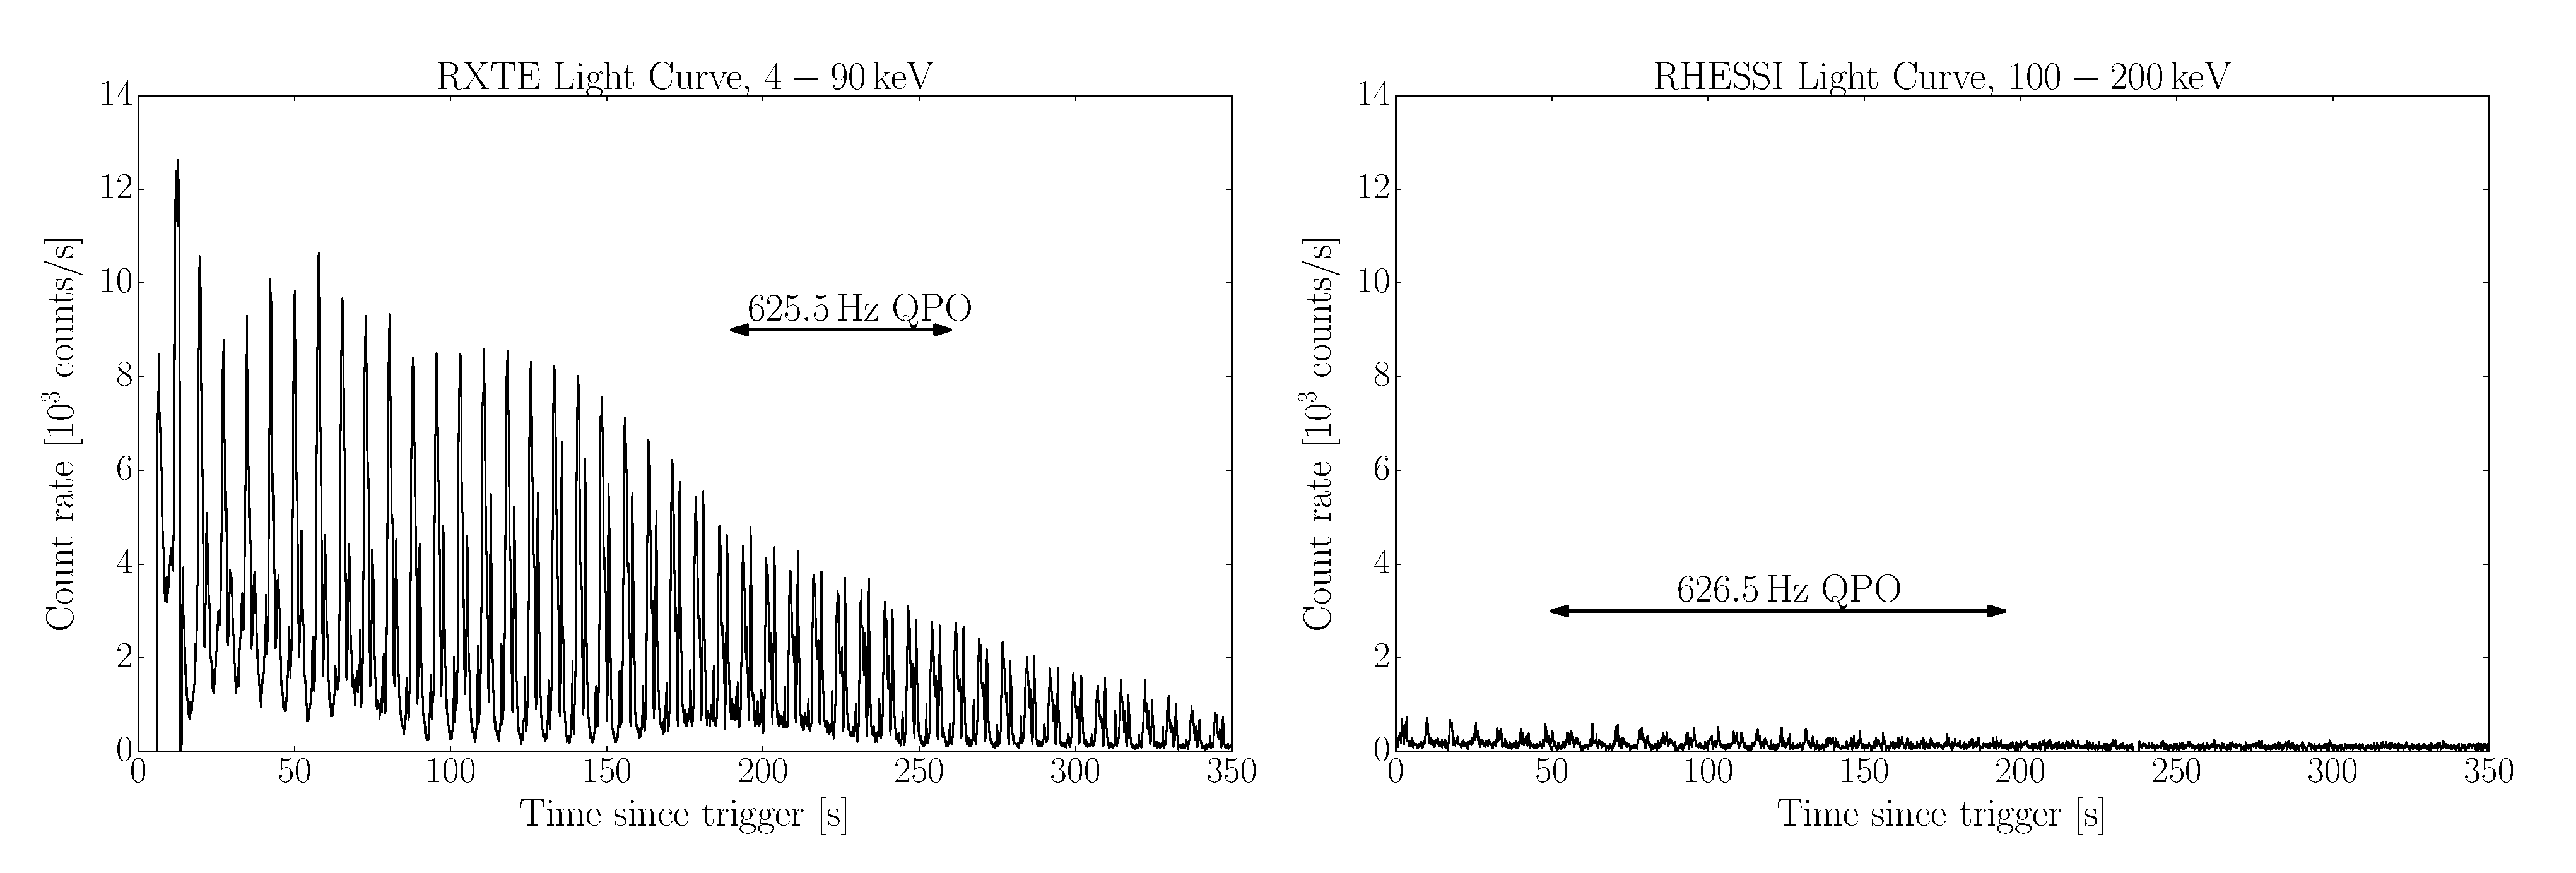
\includegraphics[width=18cm]{lightcurves.eps}
\caption{}
\label{fig:lcs}
\end{center}
\end{figure*}

\subsection{RXTE}
\label{sec:rxte_results}

\begin{figure}[htbp]
\begin{center}
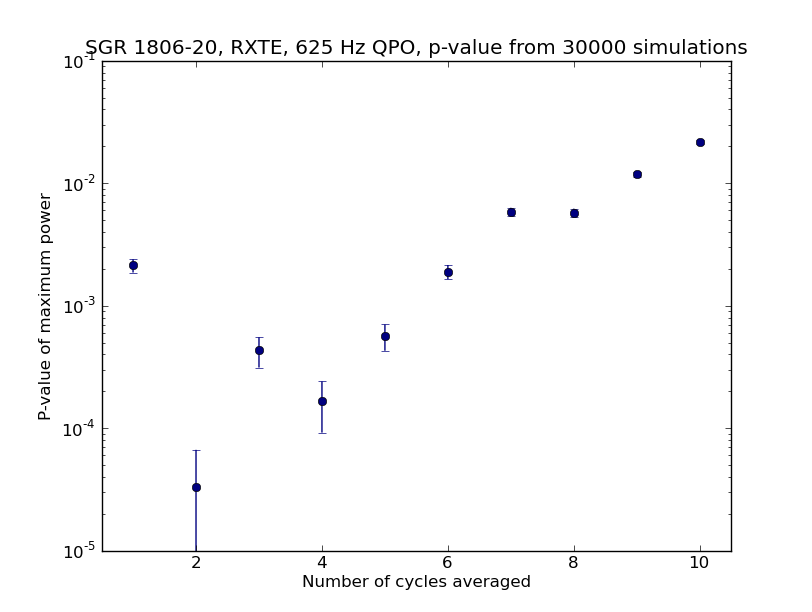
\includegraphics[width=9cm]{1806_rxte_pvals.png}
\caption{default}
\label{fig:rxte_pvals}
\end{center}
\end{figure}

\citealt{Strohmayer06} reported a detection of a strong QPO when averaging nine consecutive cycles to a significance of $p < 1.1 \times 10^{-7}$ single-trial, or $10^{-5}$ trial-corrected, and a fractional rms amplitude of $8.5\%$. These values are based on comparing the observed power to a theoretical Poisson distribution after dividing out a model fit for the low-frequency powers. They also report the detection of the same feature in an averaged periodogram of specific two cycles from the segment where the QPO was found originally with $p < 1.1 \times 10^{-6}$ single-trial and a fractional rms amplitude of $18.3\%$. A third averaged periodogram six cycles before the previous one showed a signal to $p < 4.4 \times 10^{-6}$ (single-trial), but no trial-corrected $p$-value was calculated for either of the last two reported detections, thus estimating the actual significance of these latter two signals, as compared to the nine-cycle average, is impossible.

We first repeated the analysis from \citealt{Strohmayer06} in order to reproduce their results, paying special attention to the overall number of cycles during which the signal was present, as well as the duration of the presence of the QPO in any individual cycle.
We search individual segments of $t_{\mathrm{set}} = 3 \, \mathrm{s}$ length, starting every $0.5 \, \mathrm{s}$, such that consecutive segments overlap by $2.5 \, \mathrm{s}$. We extracted the power at $625 \, \mathrm{Hz}$, then ran 30000 simulations as described in \ref{sec:analysis} and compared the powers at $625 \, \mathrm{Hz}$ for each segment as well as phase-averaged segments to the powers extracted in the same way from the simulations.

\begin{figure*}[htbp]
\begin{center}
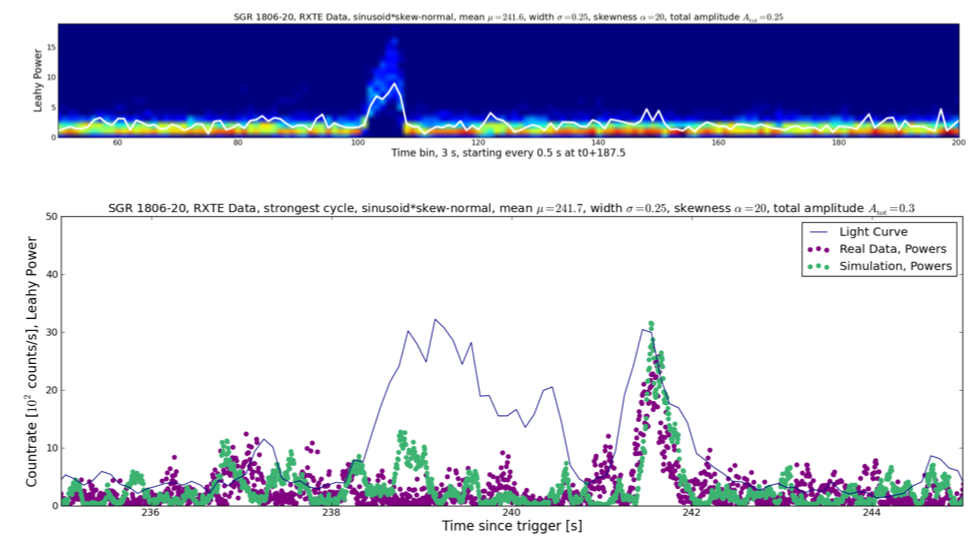
\includegraphics[width=\textwidth]{1806_rxte_lc_combined.png}
\caption{Probability of observing a signal at $625 \, \mathrm{Hz}$ in the {\it RXTE} data at least as high or higher than the observed power in dependence of the number of cycles averaged. For each data point, we extracted the maximum power from all (averaged) segments over the entire length of the searched part of the giant flare light curve, for both the observation and the simulated light curves. Errors on the p-values are derived from the theoretical approximation valid for small probabilities $\Delta p = \sqrt{p (1-p)/N}$, where $p$ is the $p-value$ and $N$ is the number of simulations. A smaller $p$-value corresponds to a higher significance: when averaging cycles, the signal actually becomes less significance, with a minimum for averaging two consecutive cycles. This indicates that the signal is likely only present in two cycles.}
\label{fig:rxte_lc_combined}
\end{center}
\end{figure*}


There is a strong QPO signal at $625$ Hz in a cycle starting at $239\, \mathrm{s}$ after the trigger, as reported in \citet{Strohmayer06}. In order to answer the question whether this signal is present over all nine cycles, for which results are reported in \citet{Strohmayer05}, or whether it is only present in a single cycle, we constructed phase-averaged periodograms averaging up to nine periodograms, and constructed p-values as described in Section \ref{sec:analysis}. Figure \ref{fig:rxte_pvals} presents the results: the QPO is significant when averaging together up to $9$ cycles to $p < 0.02$. However, we also note that the signal is most significant when averaging the cycle with the strongest signal and the immediately previous cycle together. This indicates that the QPO is likely to be present at least in these two cycles. When averaging more than two cycles, the significance drops (the p-value rises, i.e. the null hypothesis, pure noise and no QPO, becomes more likely), indicating that with every additional cycle, we are averaging in more noise rather than more signal. We conclude that the signal is most likely present in two cycles at most.
We also note that we fail to reproduce the marginal detection of a QPO at the same frequency six cycles before the cycle with the strongest incarnation of the $625\, \mathrm{Hz}$ QPO. 

Given that the QPO is likely confined to two cycles, it is reasonable to ask whether the QPO extends over both cycles, i.e. is present for the entire $\sim 14\, \mathrm{s}$, or is being re-excited. To test this, we attempted to constrain the width of the QPO in the strongest cycle. First, we redid the analysis described above, but with time segments starting exactly one cycle of the $625 \, \mathrm{Hz}$ QPO apart, i.e. every $1/625 = 1.6 \times 10^{-3} \, \mathrm{s}$ apart, effectively providing a finely resolved sliding window over the cycle where the QPO is strongest. If one then plots the strength of the signal with time, one can track the strength of the QPO over the course of the star's rotational cycle. As more signal is included in a given segment, the power will rise, until the entire signal is included. Similarly, as the sliding window moves out of the time frame where the QPO is located, less and less signal is included, and the power drops. We show the resulting plot in Figure \ref{fig:rxte_combined}. Similarly to Figure 3 in \citet{Strohmayer06}, the QPO seems to be present only on the declining edge of the second pulse, and only for a short period of time. We then injected an artificial sinusoidal signal into a single cycle in 50 simulations, in the same part of the rotational cycle as the real QPO, for a duration of $0.25\, \mathrm{s}$ and a fractional rms amplitude of $0.3$. The sinusoid is on top of a fast-rise exponential decay profile, to simulate the effect of a suddenly appearing, then decaying signal. We show a single realisation in the lower panel of Figure \ref{fig:rxte_combined}. In the upper panel, we show an image of the simulations, with data over plotted. The data traces the simulations as well, indicating that the observed QPO can be well modelled with a short, decaying, but high-amplitude QPO signal. 


\subsection{RHESSI}
\label{sec:rhessi_results}

\citealt{Watts06} searched segments of $t_{\mathrm{seg}} = 2.27$ seconds length, i.e. $1/3$ of the neutron star's rotational cycle, over a range of 19 successive cycles, starting $\sim 80 \, \mathrm{s}$ after the onset of the giant flare. They report the detection of a QPO at $626.5 \, \mathrm{Hz}$ with a significance of $6.6 \times 10^{-5}$, corrected for the number of trials, in this averaged periodogram when comparing to the theoretically expected distribution of powers for pure Poisson noise.

While previous studied constrained themselves to a single (arbitrary) segment length, we varied the length of the segments between $t_{\mathrm{seg}} = 0.5 \, \mathrm{s}$ and $t_{\mathrm{seg}} = 2.0 \, \mathrm{s}$ in our re-analysis of the {\it RHESSI} data in order to be sensitive to shorter signals, which may be buried in noise when taking the periodogram over too long a segment. This is not necessary for the {\it RXTE} data, since the signal is strong enough and the data is of high enough quality for the signal to be clearly observable even if it is considerably shorter than the segment length. For less strong signals and data of lower quality, a short signal can potentially be buried under the noise when looking at segments that are much longer compared to the duration of the QPO. 

We subdivided each cycle into $N_\mathrm{s} = 30$ segments, such that they start every $d t_\mathrm{seg}= 7.6022/30 = 0.2534 \, \mathrm{s}$ apart, and overlap for $\delta t_\mathrm{seg} - 0.2534 \, \mathrm{s}$. Again, we use a higher number of segments per cycle to account for the poorer quality of the {\it RHESSI} data, and the fact we search shorter segments: for $15$ segments per cycle, the shortest segments will not overlap at all, and a signal split between two segments may not be detected at all.
For each segment we computed the periodogram and extracted the power at $626.5 \, \mathrm{Hz}$, and compared this power to those at the same frequency from segments of 10000 simulated light curves with the giant flare pulse profile, but smoothed out such that the QPO is removed. The $p$-values for an observed power in any segment to be higher than the power in any simulated segment is shown in Figure \ref{fig:rhessi_pvalues}. If the signal is present in only one or two cycles, then the significance should decrease with increasing number of averaged cycles, since any additional cycle included in the average will only supply noise. On the other hand, if the signal is long-lived and persists over many cycles, then averaging more cycles should make the observed signal more significant. Interestingly, both behaviours are observed: for the shortest segments with $0.5\, \mathrm{s}$ length, the power observed from the giant flare is significant to $p < 0.01$ when averaging only two cycles, and remains roughly at this level or rises again as more cycles are averaged, indicating that these cycles do not supply any power to the averaged periodogram. On the other hand, for longer segments, the signal becomes more significant as more cycles are included in the averaged periodogram. One possible explanation for this behaviour is a signal that shifts in phase over the duration of the giant flare: if the QPO appears in many cycles, but is short-lived in each cycle ($<1.0 \, \mathrm{s}$) and the QPO onset moves in phase with each cycle, then the QPOs from several cycles would only add up and produce a stronger QPO in the longer segments, but not in the shorter segments, where they are distributed in different segments for different phases. 

\begin{figure}[htbp]
\begin{center}
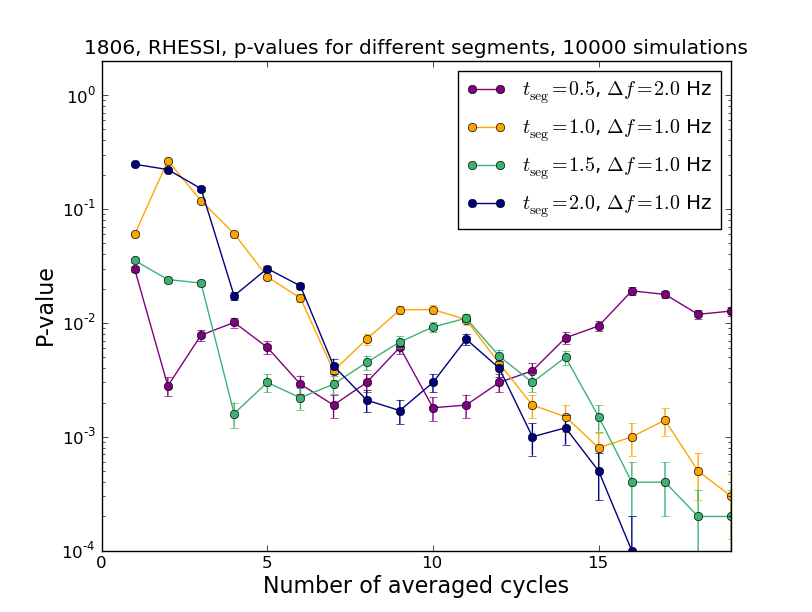
\includegraphics[width=9cm]{1806_rhessi_pvalues.png}
\caption{RHESSI data: p-values for measuring a power at $626.5\, \mathrm{Hz}$ in any of the segments at least as high or higher than the ensemble of powers derived from all segments from 10000 simulations. We show these p-values in dependence of the number of phase-matched periodograms averaged to construct the power in that segment, for different segment lengths between $0.5$ and $2.0$ seconds. The p-values for the shortest segments indicates that there is a significant signal ($p < 0.01$) even when averaging only two cycles together, while averaging in more cycles seems to supply no additional signal. For longer segments, averaging in more cycles increases the significance, indicating that the signal is longer-lived.}
\label{fig:rhessi_pvalues}
\end{center}
\end{figure}

If the signal is present in only one or two cycles, then the significance should decrease with increasing number of averaged cycles, since any additional cycle included in the average will only supply noise. On the other hand, if the signal is long-lived and persists over many cycles, then averaging more cycles should make the observed signal more significant. Interestingly, both behaviours are observed: for the shortest segments with $0.5\, \mathrm{s}$ length, the power observed from the giant flare is significant to $p < 0.01$ when averaging only two cycles, and remains roughly at this level or rises again as more cycles are averaged, indicating that these cycles do not supply any power to the averaged periodogram. On the other hand, for longer segments, the signal becomes more significant as more cycles are included in the averaged periodogram. One possible explanation for this behaviour is a signal that shifts in phase over the duration of the giant flare: if the QPO appears in many cycles, but is short-lived in each cycle ($<1.0 \, \mathrm{s}$) and the QPO onset moves in phase with each cycle, then the QPOs from several cycles would only add up and produce a stronger QPO in the longer segments, but not in the shorter segments, where they are distributed in different segments for different phases. 

\section{Simulating Signals to Understand the {\it RHESSI} Results}

Because the signal-to-noise ratio is much lower for the RHESSI data than the RXTE data, we cannot repeat the analysis of Section \ref{sec:rxte_results}, where we searched for the presence of the $626.5 \, \mathrm{Hz}$ QPO in a single cycle to a very high phase resolution in order to determine its properties, on this data set. Instead, we simulate giant flare light curves from the original data set, with the $626.5 \, \mathrm{Hz}$ QPO smoothed out, and a signal at the same frequency injected back with varying parameters. We then compute p-values for the power at $626.5 \, \mathrm{Hz}$ in the same way as for the observed giant flare data, and compare these simulated p-values with those derived from the data. We test whether the data are consistent with three different hypotheses: (1) the QPO appears at the same phase in every rotational cycle, and is consistently present over all nineteen averaged cycles; (2) the signal is present in all 19 cycles, but that its onset changes in phase between rotational cycles; (3) the signal is present in a small subset of cycles.

\subsection{Is the QPO present at the same phase in all cycles?}

In order to test the first hypothesis, we injected a sinusoidal signal at the same rotational phase ($2.07/(2\pi)$, i.e. the same rotational phase of the neutron star at which the QPO is observed in the shortest segments) for all $19$ rotational cycles we searched. The phases of the sinusoidal signal were randomised in each cycle, as well as in each simulated light curve. The resulting time series were randomised using a Poisson distribution to account for photon counting noise, and subjected to the same analysis procedure as the giant flare data to extract p-values in dependence of the number of rotational cycles averaged, for four different time segment sizes.

\begin{figure*}[htbp]
\begin{center}
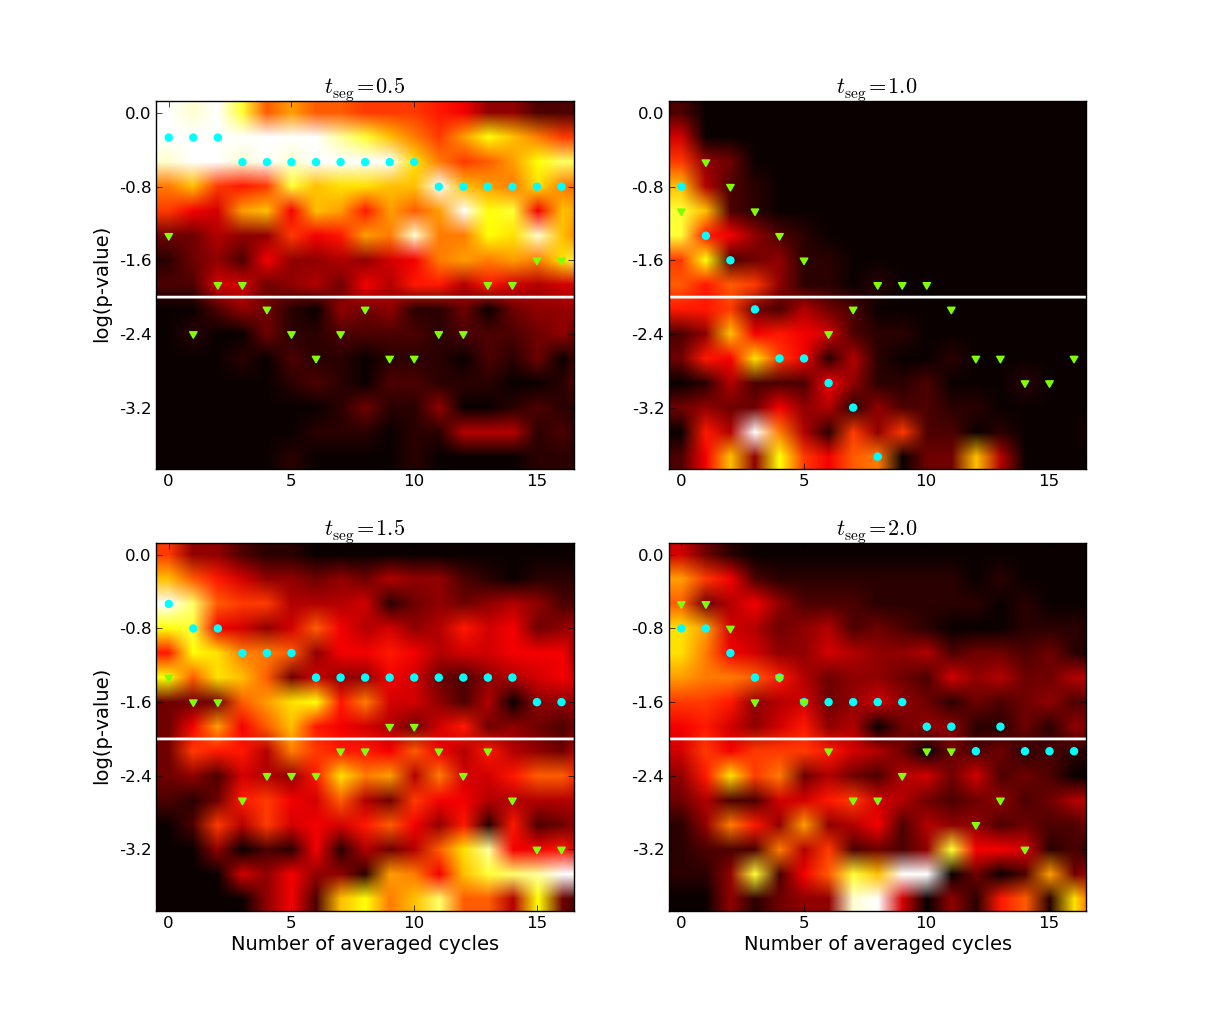
\includegraphics[width=\textwidth]{1806_rhessi_1ssignal_all_pvalues.png}
\caption{RHESSI data: observed p-values versus $100$ simulations for different segment lengths. The colour map in the background corresponds encodes the p-value that simulated light curves with a QPO of $1$ second duration and a fractional rms amplitude of $20\%$ in ever rotational cycle is likely to have in dependence of the number of averaged cycles. We plot the mean p-values from the simulations as blue circles to guide the eye; the p-values derived from the RHESSI data are shown as green triangles.}
\label{fig:rhessi_sims1_pvalues}
\end{center}
\end{figure*}

In Figure \ref{fig:rhessi_sims1} we show representative results for $100$ simulations with a QPO in every cycle of $1$ second duration and a fractional rms amplitude of $20\%$. Qualitatively, the simulations show similar p-values to the observed RHESSI data for the longer segments, whereas for $1$-second segments, the significance of the signal is overestimated. On the other hand, the QPO in the $0.5$-second segments is strongly underestimated. 
We repeated the same procedure with signals of duration of $0.5$ to $2.0$ seconds as well as varying fractional rms amplitudes. In no case could we reproduce the observed p-values: the simulations either drastically underestimate the p-values for the shortest segments, or drastically overestimate the p-values in the longer segments. 
This is not unexpected: in order to reproduce a signal of the observed p-value $p = 3.9 \times 10^{-3}$ in two consecutive cycles, we require a very high fractional rms amplitude in excess of $70\%$. While the resulting QPO will be less significant in the longer segments (as more background noise is included in the periodogram), averaging over many cycles yields a QPO that is much more significant than the observations suggest. On the other hand, decreasing the fractional rms amplitude to a level where the behaviour in the longer segment matches yields p-values for the shortest segments that are much too high. 

 
\subsection{Is the QPO present in all rotational cycles at different phases?}

As a second test, we checked whether the signal could be present in all nineteen cycles, but shifting in rotational phase of the neutron star. We injected a signal of $1.0\, \mathrm{s}$ duration and $22\%$ fractional rms amplitude into every cycle, with the start time of the QPO varying randomly from cycle to cycle in a 1-second interval around phase $0.66\pi$. We created 100 light curves in this way, each of which was randomised using a Poisson distribution to account for photon detector noise. Each of these light curves was run through the analysis procedure to extract p-values in the same way as the real data and the preceding section. 
The resulting distribution of p-values is given in Figure \ref{fig:rhessi_sims2_pvalues}. We find these simulations to be a closer match in qualitative change of the p-values with segment length and number of averaged cycles than the simulations with equal phase are. Note that the behaviour for the shortest segments is still noticeably different from what is seen in the data: the p-value decreases to higher significance with increasing number of cycles, as opposed to the increasing p-value in the observed data. This may indicate that the signal may be shorter in duration than we have injected here, or that it may jump even more in phase. Additionally, the QPO in the observed data requires a much higher fractional rms amplitude in at least one or two cycles, indicating that the fractional rms amplitude changes throughout the giant flare.
The longer segments all match up fairly well in general; however, especially for the longest segments there is an increase in the p-values when averaging between $5$ and $10$ cycles together; perhaps the signal is not present throughout the entire segment, but rather re-appears in the last stages of the giant flare.


\begin{figure*}[htbp]
\begin{center}
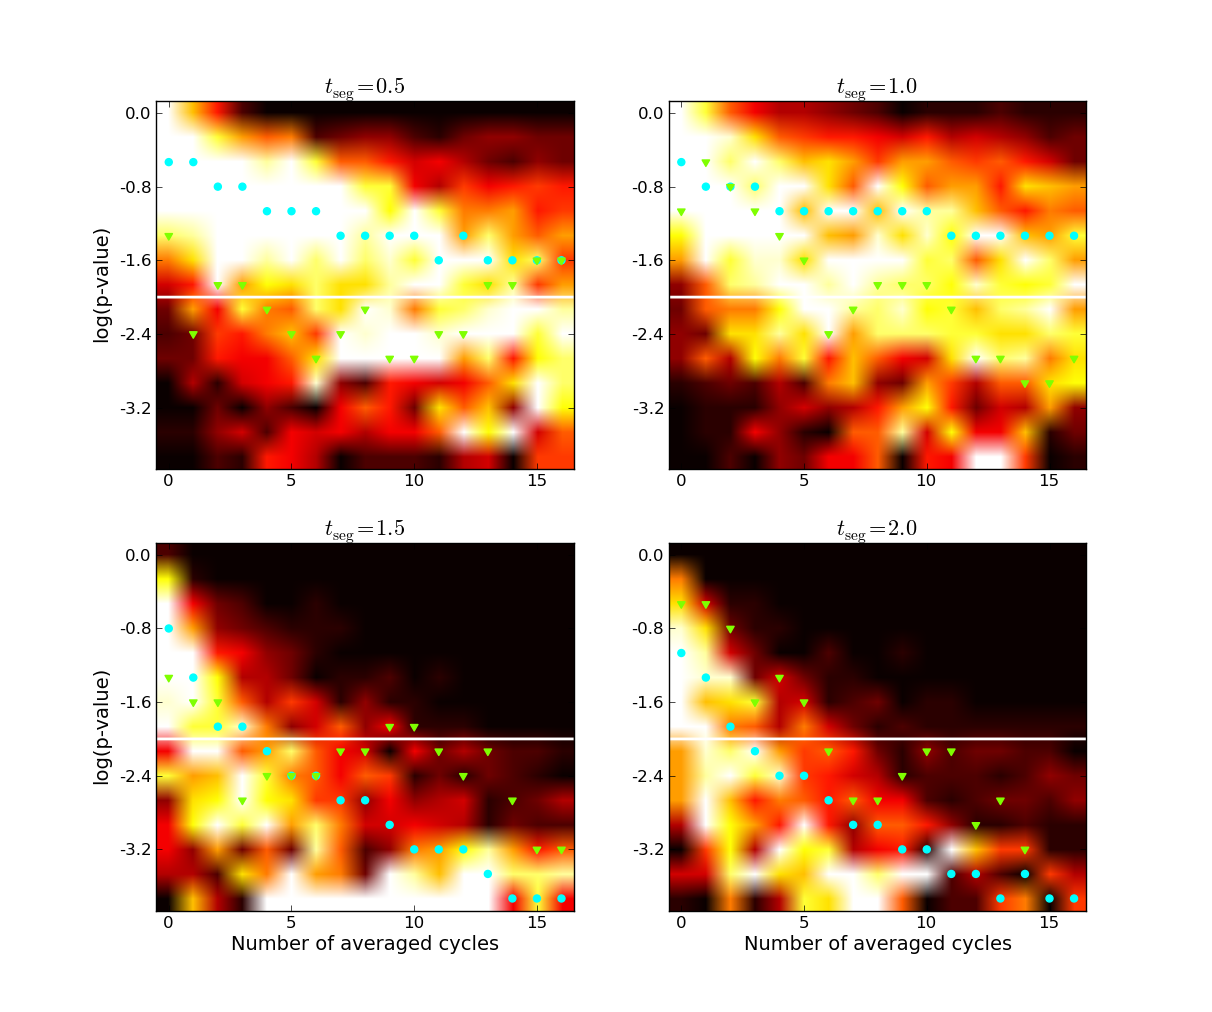
\includegraphics[width=\textwidth]{1806_rhessi_1ssignal_randomphase_pvalues.png}
\caption{RHESSI data: observed p-values versus $100$ simulations for different segment lengths. The colour map in the background corresponds encodes the p-value that simulated light curves with a QPO of $1$ second duration and a fractional rms amplitude of $20\%$ is likely to have in dependence of the number of averaged cycles. We plot the mean p-values from the simulations as blue circles to guide the eye; the p-values derived from the RHESSI data are shown as green triangles.}
\label{fig:rhessi_sims2_pvalues}
\end{center}
\end{figure*}


\subsection{Is the observed QPO with a signal present in a few cycles?}

Testing whether the QPO is only present in few cycles is not straightforward with the kind of forward-fitting technique employed here: a QPO that could be present in any number of the 19 cycles considered here, and no potential QPO duration per rotational cycle or QPO amplitude can be excluded a priori. This leaves us with an enormous parameter space to traverse, while at the same time creating a large number of simulations and performing the same analysis as on the data for each possible parameter set becomes prohibitively expensive. We thus restrict ourselves with few informed guesses to the possible distribution of QPOs, and with qualitative arguments for the simulations we considered. 

We injected a strong, short signal (segment length $0.5\,\mathrm{s}$, fractional rms amplitude $75\%$) into the same cycle and at the same phase as the strongest single-cycle signal in the observed data, as well as a somewhat weaker QPO ($50\%$ fractional rms amplitude) into the following cycle to approximate the strong signal seen in the shortest segments. Additionally, we injected a signal of $1\,\mathrm{s}$ duration into the last five cycles of our simulated light curves to approximate the behaviour of the observed p-values in the longer segments. We simulated $100$ light curves in the same way as in the preceding two sections, and computed p-values for each in the same way as for the observed giant flare data. The resulting distributions of p-values for the different segments and number of averaged cycles are presented in Figure \ref{fig:rhessi_sims3_pvalues}. We note that unlike for the two preceding sets of simulations, the scatter here is extremely large, to the point where it is nearly impossible to draw any strong conclusions, especially for segments of $0.5\, \mathrm{s}$ and $1.5 \, \mathrm{s}$. This may be in part caused by the fact that we introduced the longer, weaker signals into the last part of the giant flare light curve, where the signal-to-noise ratio is small and Poisson statistics noticeably affect the detectability of a QPO.
Introducing a short, very strong signal in a single cycle will cause a similarly strong detection in the longer segments as well, leading to p-values that are of higher significance than is observed in the data. On the other hand, a signal only present in five rotational cycles in the last part of the giant flare will not adequately reproduce the p-values in the longer segments of the observed data, indicating that the signal may be there for longer, or perhaps should re-appear earlier in the giant flare.

\begin{figure*}[htbp]
\begin{center}
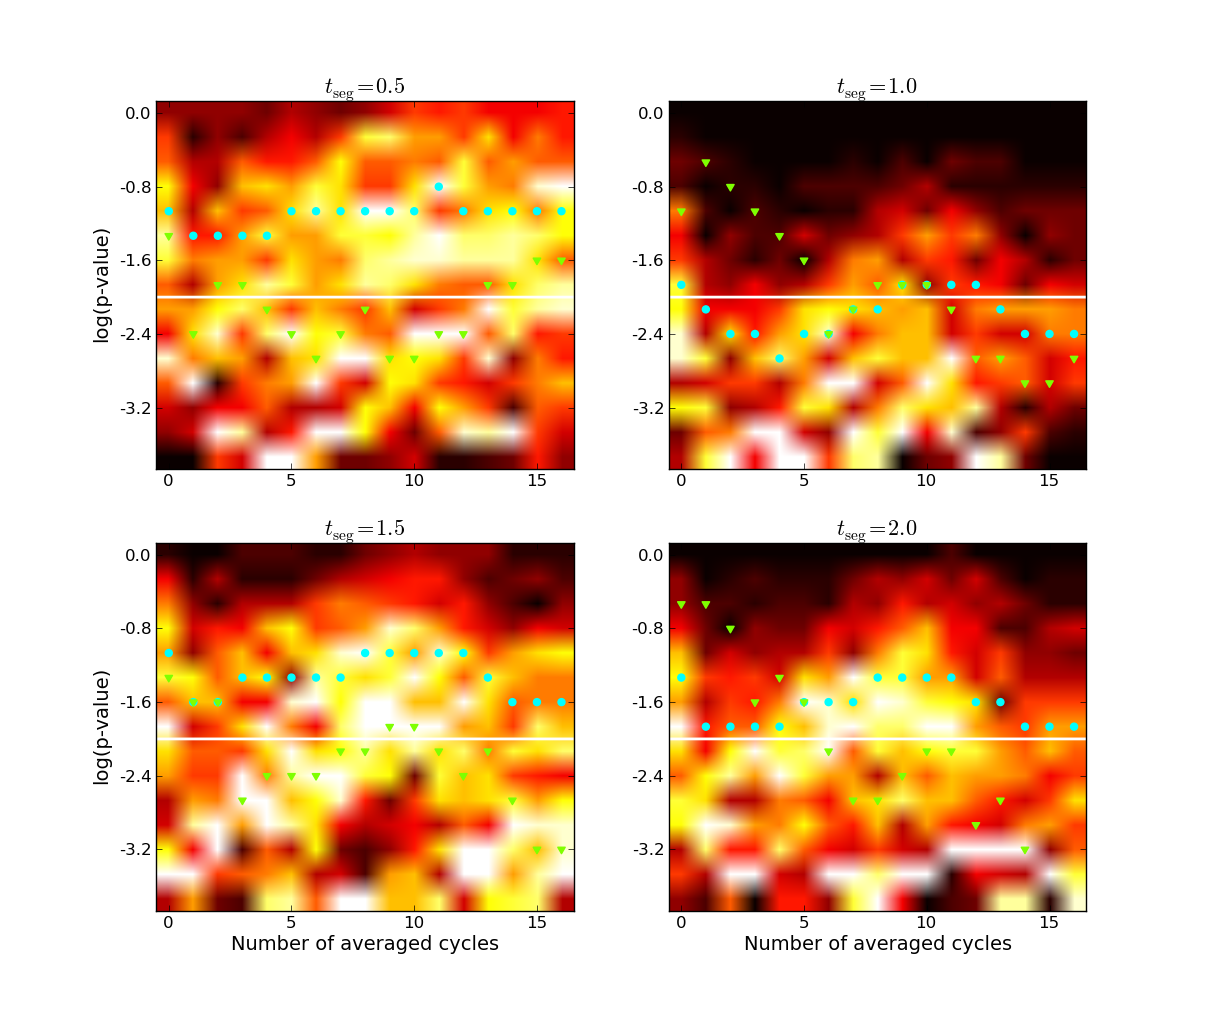
\includegraphics[width=\textwidth]{1806_rhessi_somesignals_pvalues.png}
\caption{RHESSI data: observed p-values versus $100$ simulations for different segment lengths. The colour map in the background corresponds encodes the p-value that simulated light curves with a QPO of $1$ second duration and a fractional rms amplitude of $20\%$ is likely to have in dependence of the number of averaged cycles. We plot the mean p-values from the simulations as blue circles to guide the eye; the p-values derived from the RHESSI data are shown as green triangles.}
\label{fig:rhessi_sims3_pvalues}
\end{center}
\end{figure*}




\section{Discussion}
\label{sec:discussion}

\bibliography{bibliography}
\bibliographystyle{apj}

\end{document}
